\documentclass{article}

% content/resources/templates/preamble.tex
\usepackage[margin=0.6in]{geometry}
\author{Milav Dabgar}
\usepackage{amsmath,amssymb,amsthm}
\usepackage{booktabs}
\usepackage{multirow}
\usepackage{xcolor}
\usepackage{tcolorbox}
\tcbuselibrary{breakable,skins}
\usepackage[colorlinks=true,linkcolor=blue]{hyperref}
\usepackage{titlesec}
\usepackage{enumitem}
\usepackage{tikz}
\usepackage{pgfplots}
\usepackage{circuitikz}
\usepackage[version=4]{mhchem}
\usepackage{longtable}
\usepackage{array}
\usepackage{float}
\usepackage{caption}
\usepackage{listings}

\lstset{
  basicstyle=\small\ttfamily,
  breaklines=true,
  breakatwhitespace=false,
  postbreak=\mbox{\textcolor{red}{$\hookrightarrow$}\space},
  float=false,
  numbers=left,
  numberstyle=\tiny\color{gray},
  numbersep=10pt,
  xleftmargin=2em,
  keywordstyle=\color{blue},
  commentstyle=\color{green!60!black},
  stringstyle=\color{purple},
  backgroundcolor=\color{gray!5},
  showstringspaces=false,
  tabsize=2,
  captionpos=b,
  keepspaces=true,
  columns=flexible
}

\pgfplotsset{compat=1.18}
\usetikzlibrary{shapes,arrows,positioning,calc,patterns,decorations.pathmorphing,decorations.markings,arrows.meta}

% Color scheme
\definecolor{headcolor}{RGB}{0,102,204}
\definecolor{keycolor}{RGB}{220,20,60}
\definecolor{solutioncolor}{RGB}{34,139,34}
\definecolor{mnemoniccolor}{RGB}{148,0,211}
\definecolor{codecolor}{RGB}{0,0,100}

% Spacing
\setlength{\parskip}{3pt}
\setlist[itemize]{nosep}
\setlist[enumerate]{nosep}

% Title formatting
\titleformat{\section}{\Large\bfseries\color{headcolor}}{\thesection}{1em}{}
\titleformat{\subsection}{\large\bfseries\color{headcolor}}{\thesubsection}{1em}{}

% Pandoc tightlist compatibility
\providecommand{\tightlist}{%
  \setlength{\itemsep}{0pt}\setlength{\parskip}{0pt}}

% Pandoc longtable compatibility
\newcounter{none}
\def\thenone{}


% content/resources/templates/english-boxes.tex

% Custom environments
\newtcolorbox{solutionbox}{
 breakable,
 enhanced,
 colback=solutioncolor!5!white,
 colframe=solutioncolor!75!black,
 fonttitle=\bfseries,
 title=Solution
}

\newtcolorbox{solutionboxnobreak}{
 colback=solutioncolor!5!white,
 colframe=solutioncolor!75!black,
 fonttitle=\bfseries,
 title=Solution
}

\newtcolorbox{keyformula}{
 breakable,
 enhanced,
 colback=keycolor!5!white,
 colframe=keycolor!75!black,
 fonttitle=\bfseries,
 title=Key Formula
}

\newtcolorbox{mnemonicboxenv}{
 breakable,
 enhanced,
 colback=mnemoniccolor!5!white,
 colframe=mnemoniccolor!75!black,
 fonttitle=\bfseries,
 title=Mnemonic
}

\newcommand{\mnemonicbox}[1]{%
  \begin{mnemonicboxenv}
    #1
  \end{mnemonicboxenv}
}


% Custom commands for GTU solutions
% This file defines semantic commands for consistent formatting

% Question command with automatic formatting
\newcommand{\question}[2]{%
  \section*{Question #1}%
  \textbf{#2}%
}

% OR question variant
\newcommand{\questionor}[2]{%
  \section*{Question #1 OR}%
  \textbf{#2}%
}

% Proper table environment with caption
\newenvironment{answertable}[1]{%
  \begin{table}[htbp]
  \centering
  \caption{#1}
}{%
  \end{table}
}

% Proper figure environment for diagrams
\newenvironment{answerdiagram}[1]{%
  \begin{figure}[htbp]
  \centering
  \caption{#1}
}{%
  \end{figure}
}

% Semantic markup for key terms
\newcommand{\keyword}[1]{\textbf{#1}}
\newcommand{\code}[1]{\texttt{#1}}
\newcommand{\classname}[1]{\texttt{#1}}
\newcommand{\methodname}[1]{\texttt{#1}}

% Proper quotation marks
\newcommand{\mnemonic}[1]{``#1''}


\title{Digital \& Data Communication (4343201) - Winter 2024 Solution}
\date{November 26, 2024}

\begin{document}
\maketitle

\questionmarks{1(a)}{3}{Differentiate Basic modes of Communication: Broad casting communication and Point to Point Communication.}

\begin{solutionbox}
\begin{center}
\captionof{table}{Broadcasting vs Point-to-Point}
\begin{tabulary}{\linewidth}{|L|L|L|}
\hline
\textbf{Parameter} & \textbf{Broadcasting Communication} & \textbf{Point to Point Communication} \\ \hline
\textbf{Definition} & One transmitter sends signals to multiple receivers simultaneously & One transmitter communicates with one specific receiver \\ \hline
\textbf{Direction} & Unidirectional (one-way) & Bidirectional (two-way) \\ \hline
\textbf{Examples} & TV, Radio, FM & Telephone, Mobile calls, Private networks \\ \hline
\textbf{Privacy} & Low (signal available to everyone in range) & High (dedicated connection between endpoints) \\ \hline
\textbf{Efficiency} & High for mass communication & Better for personal/private communication \\ \hline
\end{tabulary}
\end{center}

\begin{itemize}
    \item \keyword{Broadcasting}: Targeted at mass audience (One-to-Many).
    \item \keyword{Point-to-Point}: Targeted at specific individual (One-to-One).
\end{itemize}
\end{solutionbox}

\begin{mnemonicbox}
\mnemonic{BDPEC - Broadcasting Distributes to Public, Endpoints Connect in point-to-point}
\end{mnemonicbox}

\questionmarks{1(b)}{4}{Define: Bit Rate, Baud Rate, Bandwidth and Repeater Distance.}

\begin{solutionbox}
\begin{center}
\captionof{table}{Definitions}
\begin{tabulary}{\linewidth}{|L|L|}
\hline
\textbf{Term} & \textbf{Definition} \\ \hline
\textbf{Bit Rate} & Number of binary bits transmitted per second (bps). Measures actual data transfer speed. \\ \hline
\textbf{Baud Rate} & Number of signal units or symbols transmitted per second. One symbol may contain multiple bits. \\ \hline
\textbf{Bandwidth} & Range of frequencies used by a signal, measured in Hertz (Hz). Determines maximum data capacity of a channel. \\ \hline
\textbf{Repeater Distance} & Maximum distance between repeaters in a communication system before signal degradation requires regeneration. \\ \hline
\end{tabulary}
\end{center}

\begin{center}
\begin{tikzpicture}[node distance=1.5cm, auto]
    \node [gtu block] (sig) {Signal};
    \node [gtu block, right=2cm of sig] (bw) {Bandwidth};
    \node [gtu block, below=1cm of sig] (bits) {Bits};
    \node [gtu block, right=2cm of bits] (br) {Bit Rate};
    \node [gtu block, below=1cm of bits] (sym) {Symbols};
    \node [gtu block, right=2cm of sym] (baurd) {Baud Rate};
    
    \draw [gtu arrow] (sig) -- node {freq range} (bw);
    \draw [gtu arrow] (bits) -- node {per sec} (br);
    \draw [gtu arrow] (sym) -- node {per sec} (baurd);
\end{tikzpicture}
\captionof{figure}{Communication Rate Concepts}
\end{center}
\end{solutionbox}

\begin{mnemonicbox}
\mnemonic{BBRR - Better Bandwidth Requires Repeaters}
\end{mnemonicbox}

\questionmarks{1(c)}{7}{Draw the block diagram of digital communication system. Explain the functions of each block in brief. State advantages and disadvantages of it.}

\begin{solutionbox}
\begin{center}
\begin{tikzpicture}[node distance=1.5cm, auto, font=\small]
    \node [gtu block] (source) {Input Source};
    \node [gtu block, right=0.8cm of source] (senc) {Source Encoder};
    \node [gtu block, right=0.8cm of senc] (cenc) {Channel Encoder};
    \node [gtu block, right=0.8cm of cenc] (mod) {Digital Modulator};
    
    \node [gtu block, below=1.5cm of mod] (channel) {Channel};
    \node [gtu block, below=1.5cm of channel] (demod) {Digital Demodulator};
    \node [gtu block, left=0.8cm of demod] (cdec) {Channel Decoder};
    \node [gtu block, left=0.8cm of cdec] (sdec) {Source Decoder};
    \node [gtu block, left=0.8cm of sdec] (dest) {Output};
    
    \draw [gtu arrow] (source) -- (senc);
    \draw [gtu arrow] (senc) -- (cenc);
    \draw [gtu arrow] (cenc) -- (mod);
    \draw [gtu arrow] (mod) -- (channel);
    \draw [gtu arrow] (channel) -- (demod);
    \draw [gtu arrow] (demod) -- (cdec);
    \draw [gtu arrow] (cdec) -- (sdec);
    \draw [gtu arrow] (sdec) -- (dest);
\end{tikzpicture}
\captionof{figure}{Digital Communication System}
\end{center}

\begin{itemize}
    \item \keyword{Source Encoder}: Converts analog signal to digital, removes redundancy, compresses data.
    \item \keyword{Channel Encoder}: Adds redundancy for error detection and correction.
    \item \keyword{Digital Modulator}: Converts digital data to suitable form for transmission (ASK, FSK, PSK).
    \item \keyword{Channel}: Medium through which signal travels (wired/wireless).
    \item \keyword{Digital Demodulator}: Extracts original digital data from received modulated signal.
    \item \keyword{Channel Decoder}: Detects and corrects errors using added redundancy.
    \item \keyword{Source Decoder}: Decompresses data and converts to original form.
\end{itemize}

\begin{center}
\captionof{table}{Advantages and Disadvantages}
\begin{tabulary}{\linewidth}{|L|L|}
\hline
\textbf{Advantages} & \textbf{Disadvantages} \\ \hline
Better noise immunity & Requires more bandwidth \\ \hline
Easier signal regeneration & Complex implementation \\ \hline
Secure transmission possible & Synchronization required \\ \hline
Integration with computers & Quantization errors \\ \hline
Better quality for long distance & Higher cost for simple applications \\ \hline
\end{tabulary}
\end{center}
\end{solutionbox}

\begin{mnemonicbox}
\mnemonic{SECDCSO - Secure Encoding Creates Digital Communication System Output}
\end{mnemonicbox}

\questionmarks{1(c OR)}{7}{Justify the needs of multiplexing techniques for digital communication. Draw and explain Time Division multiplexing technique in brief. Discuss its merits and demerits.}

\begin{solutionbox}
\textbf{Need for Multiplexing:}
\begin{center}
\captionof{table}{Need for Multiplexing}
\begin{tabulary}{\linewidth}{|L|L|}
\hline
\textbf{Need} & \textbf{Explanation} \\ \hline
\textbf{Channel Efficiency} & Allows multiple signals on one channel, saving bandwidth \\ \hline
\textbf{Cost Reduction} & Reduces need for multiple transmission media \\ \hline
\textbf{Infrastructure Utilization} & Maximizes use of expensive infrastructure \\ \hline
\textbf{Spectrum Conservation} & Conserves limited frequency spectrum \\ \hline
\end{tabulary}
\end{center}

\textbf{Time Division Multiplexing (TDM):}
\begin{center}
\begin{tikzpicture}[node distance=1.5cm, auto]
    \node [gtu block] (mux) {Multiplexer};
    \node [gtu block, right=3cm of mux] (demux) {Demultiplexer};
    
    \node [left=1cm of mux] (in2) {Input 2};
    \node [above=0.5cm of in2] (in1) {Input 1};
    \node [below=0.5cm of in2] (in3) {Input 3};
    \node [below=0.5cm of in2] (in4) {Input 4};
    
    \node [right=1cm of demux] (out2) {Output 2};
    \node [above=0.5cm of out2] (out1) {Output 1};
    \node [below=0.5cm of out2] (out3) {Output 3};
    \node [below=0.5cm of out2] (out4) {Output 4};
    
    \draw [gtu arrow] (in1) -- (mux.west |- in1);
    \draw [gtu arrow] (in2) -- (mux.west |- in2);
    \draw [gtu arrow] (in3) -- (mux.west |- in3);
    \draw [gtu arrow] (in4) -- (mux.west |- in4);
    
    \draw [gtu arrow] (mux) -- node {Transmission Channel} (demux);
    
    \draw [gtu arrow] (demux.east |- out1) -- (out1);
    \draw [gtu arrow] (demux.east |- out2) -- (out2);
    \draw [gtu arrow] (demux.east |- out3) -- (out3);
    \draw [gtu arrow] (demux.east |- out4) -- (out4);
\end{tikzpicture}
\captionof{figure}{Time Division Multiplexing (TDM)}
\end{center}

\begin{itemize}
    \item \keyword{Working}: In TDM, each input signal gets a specific time slot. The multiplexer samples each input sequentially, combining them into a single high-speed data stream. At the receiver, signals are separated based on timing.
\end{itemize}

\begin{center}
\captionof{table}{Merits and Demerits}
\begin{tabulary}{\linewidth}{|L|L|}
\hline
\textbf{Merits} & \textbf{Demerits} \\ \hline
Efficient bandwidth usage & Requires synchronization \\ \hline
No guard bands needed & Complex buffering required \\ \hline
No cross-talk & Timing issues can cause errors \\ \hline
Flexible allocation & Unused slots waste capacity \\ \hline
Digital implementation & Higher data rate than individual channels \\ \hline
\end{tabulary}
\end{center}
\end{solutionbox}

\begin{mnemonicbox}
\mnemonic{TIME - Transmission Interleaves Multiple Endpoints}
\end{mnemonicbox}

\questionmarks{2(a)}{3}{Differentiate: Coherent and Non-Coherent Detection Technique.}

\begin{solutionbox}
\begin{center}
\captionof{table}{Coherent vs Non-Coherent Detection}
\begin{tabulary}{\linewidth}{|L|L|L|}
\hline
\textbf{Parameter} & \textbf{Coherent Detection} & \textbf{Non-Coherent Detection} \\ \hline
\textbf{Phase Information} & Uses phase information & Ignores phase information \\ \hline
\textbf{Local Oscillator} & Required & Not required \\ \hline
\textbf{Complexity} & More complex & Simpler \\ \hline
\textbf{Performance} & Better noise immunity & Less efficient in noise \\ \hline
\textbf{Implementation} & Difficult & Easier \\ \hline
\textbf{Applications} & High-quality systems & Low-cost systems \\ \hline
\end{tabulary}
\end{center}
\end{solutionbox}

\begin{mnemonicbox}
\mnemonic{PLCPIA - Phase Local Complex Performance Implementation Applications}
\end{mnemonicbox}

\questionmarks{2(b)}{4}{Sketch the ASK, FSK, PSK and QPSK waveform for the data sequence 101100110110.}

\begin{solutionbox}
\begin{center}
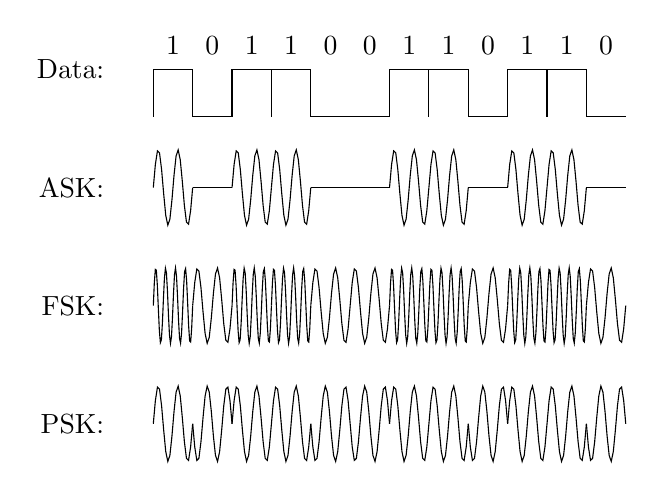
\begin{tikzpicture}[x=0.5cm,y=0.6cm]
    % Digital Data
    \node[anchor=east] at (-1, 1) {Data:};
    \foreach \x/\val in {0/1, 1/0, 2/1, 3/1, 4/0, 5/0, 6/1, 7/1, 8/0, 9/1, 10/1, 11/0} {
        \draw (\x,0) -- (\x,\val) -- (\x+1,\val) -- (\x+1,0); 
        \node at (\x+0.5, 1.5) {\val};
    }
    
    % ASK
    \node[anchor=east] at (-1, -1.5) {ASK:};
    \foreach \x/\val in {0/1, 1/0, 2/1, 3/1, 4/0, 5/0, 6/1, 7/1, 8/0, 9/1, 10/1, 11/0} {
        \ifnum\val=1
            \draw[domain=\x:\x+1, samples=20] plot (\x, {sin(360*(\x)*2) * 0.8 - 1.5});
        \else
            \draw (\x,-1.5) -- (\x+1,-1.5);
        \fi
    }
    
    % FSK
    \node[anchor=east] at (-1, -4) {FSK:};
    \foreach \x/\val in {0/1, 1/0, 2/1, 3/1, 4/0, 5/0, 6/1, 7/1, 8/0, 9/1, 10/1, 11/0} {
        \ifnum\val=1
            \draw[domain=\x:\x+1, samples=40] plot (\x, {sin(360*(\x)*4) * 0.8 - 4});
        \else
            \draw[domain=\x:\x+1, samples=20] plot (\x, {sin(360*(\x)*2) * 0.8 - 4});
        \fi
    }
    
    % PSK (Using BPSK implicitly as PSK usually refers to BPSK in exams unless specified otherwise)
    \node[anchor=east] at (-1, -6.5) {PSK:};
    \foreach \x/\val in {0/1, 1/0, 2/1, 3/1, 4/0, 5/0, 6/1, 7/1, 8/0, 9/1, 10/1, 11/0} {
        \ifnum\val=1
            \draw[domain=\x:\x+1, samples=20] plot (\x, {sin(360*(\x)*2) * 0.8 - 6.5});
        \else
            \draw[domain=\x:\x+1, samples=20] plot (\x, {-sin(360*(\x)*2) * 0.8 - 6.5});
        \fi
    }
    
\end{tikzpicture}
\captionof{figure}{Modulation Waveforms}
\end{center}

\begin{itemize}
    \item \keyword{QPSK}: Represented by phase shifts of 0, 90, 180, 270 degrees for dibits (00, 01, 10, 11).
\end{itemize}
\end{solutionbox}

\begin{mnemonicbox}
\mnemonic{AFPQ - Amplitude Frequency Phase Quadrature}
\end{mnemonicbox}

\questionmarks{2(c)}{7}{Explain the principle of 16-QAM. Also explain constellation diagram and waveform for 16-QAM. Write its advantages and disadvantages.}

\begin{solutionbox}
\textbf{Principle of 16-QAM:}
16-QAM (Quadrature Amplitude Modulation) combines amplitude and phase modulation to transmit 4 bits per symbol. It uses 16 different combinations of amplitude and phase, allowing higher data rates in the same bandwidth.

\textbf{Constellation Diagram:}
\begin{center}
\begin{tikzpicture}[scale=1.2]
    \draw[->] (-3,0) -- (3,0) node[right] {I};
    \draw[->] (0,-3) -- (0,3) node[above] {Q};
    
    \foreach \x in {-1.5, -0.5, 0.5, 1.5} {
        \foreach \y in {-1.5, -0.5, 0.5, 1.5} {
            \draw[fill] (\x,\y) circle (2pt);
        }
    }
    \node at (2, -2.5) {16 Points};
\end{tikzpicture}
\captionof{figure}{16-QAM Constellation}
\end{center}

\textbf{Waveform:}
The 16-QAM waveform varies in both amplitude (4 levels) and phase (4 phases), creating 16 unique symbols. Each point represents 4 bits (0000 to 1111).

\begin{center}
\captionof{table}{Advantages and Disadvantages}
\begin{tabulary}{\linewidth}{|L|L|}
\hline
\textbf{Advantages} & \textbf{Disadvantages} \\ \hline
High spectral efficiency & Sensitive to noise and interference \\ \hline
Higher data rate & Requires higher SNR \\ \hline
Bandwidth efficient & Complex implementation \\ \hline
Better use of channel capacity & Susceptible to amplitude distortion \\ \hline
\end{tabulary}
\end{center}
\end{solutionbox}

\begin{mnemonicbox}
\mnemonic{SCHAP - Sixteen Combinations Have Amplitude and Phase}
\end{mnemonicbox}

\questionmarks{2(a OR)}{3}{Compare: ASK and PSK}

\begin{solutionbox}
\begin{center}
\captionof{table}{ASK vs PSK}
\begin{tabulary}{\linewidth}{|L|L|L|}
\hline
\textbf{Parameter} & \textbf{ASK (Amplitude Shift Keying)} & \textbf{PSK (Phase Shift Keying)} \\ \hline
\textbf{Modulation Parameter} & Amplitude & Phase \\ \hline
\textbf{Noise Immunity} & Poor & Good \\ \hline
\textbf{Power Efficiency} & Less efficient & More efficient \\ \hline
\textbf{Bandwidth Efficiency} & Lower & Higher \\ \hline
\textbf{Implementation} & Simple & More complex \\ \hline
\textbf{BER Performance} & Higher error rate & Lower error rate \\ \hline
\end{tabulary}
\end{center}
\end{solutionbox}

\begin{mnemonicbox}
\mnemonic{ANPBIP - Amplitude Noise Power Bandwidth Implementation Performance}
\end{mnemonicbox}

\questionmarks{2(b OR)}{4}{Draw the block diagram of BPSK modulator and demodulator.}

\begin{solutionbox}
\textbf{BPSK Modulator:}
\begin{center}
\begin{tikzpicture}[node distance=1.5cm, auto]
    \node [gtu block] (nrz) {NRZ Encoder};
    \node [gtu block, right=1.5cm of nrz] (mod) {Multiplier};
    \node [above=1cm of mod] (osc) {Carrier Generator};
    \node [left=1.5cm of nrz] (in) {Binary Input};
    \node [right=1.5cm of mod] (out) {BPSK Output};
    
    \draw [gtu arrow] (in) -- (nrz);
    \draw [gtu arrow] (nrz) -- (mod);
    \draw [gtu arrow] (osc) -- (mod);
    \draw [gtu arrow] (mod) -- (out);
\end{tikzpicture}
\captionof{figure}{BPSK Modulator}
\end{center}

\textbf{BPSK Demodulator:}
\begin{center}
\begin{tikzpicture}[node distance=1.5cm, auto]
    \node [gtu block] (mult) {Multiplier};
    \node [gtu block, right=1.5cm of mult] (lpf) {Low Pass Filter};
    \node [gtu block, right=1.5cm of lpf] (dec) {Decision Device};
    
    \node [above=1cm of mult] (local) {Phase Synchronizer};
    \node [left=1cm of local] (osc) {Local Oscillator};
    
    \node [left=1.5cm of mult] (in) {BPSK Input};
    \node [right=1.5cm of dec] (out) {Binary Output};
    
    \draw [gtu arrow] (in) -- (mult);
    \draw [gtu arrow] (osc) -- (local);
    \draw [gtu arrow] (local) -| (mult);
    \draw [gtu arrow] (mult) -- (lpf);
    \draw [gtu arrow] (lpf) -- (dec);
    \draw [gtu arrow] (dec) -- (out);
\end{tikzpicture}
\captionof{figure}{BPSK Demodulator}
\end{center}
\end{solutionbox}

\begin{mnemonicbox}
\mnemonic{MNECO - Modulation Needs Encoding, Carriers, Oscillators}
\end{mnemonicbox}

\questionmarks{2(c OR)}{7}{Explain QPSK generation and detection with the help of block diagram and waveform. Discuss its advantages and disadvantages.}

\begin{solutionbox}
\textbf{QPSK Generation Block Diagram:}
\begin{center}
\begin{tikzpicture}[node distance=1.5cm, auto]
    \node [gtu block] (sp) {Serial to Parallel};
    \node [gtu block, right=2cm of sp, yshift=1cm] (mult1) {Multiplier I};
    \node [gtu block, right=2cm of sp, yshift=-1cm] (mult2) {Multiplier Q};
    \node [gtu block, right=2cm of mult1, yshift=-1cm] (adder) {Adder};
    \node [right=1cm of adder] (out) {QPSK Output};
    
    \node [left=1cm of sp] (input) {Binary Input};
    \node [above=1.5cm of sp] (osc) {Carrier Generator};
    \node [right=1cm of osc] (shift) {90° Phase Shifter};
    
    \draw [gtu arrow] (input) -- (sp);
    \draw [gtu arrow] (sp) -- node[above, sloped] {I-channel} (mult1);
    \draw [gtu arrow] (sp) -- node[below, sloped] {Q-channel} (mult2);
    
    \draw [gtu arrow] (osc) -| (mult1);
    \draw [gtu arrow] (osc) -- (shift);
    \draw [gtu arrow] (shift) -| (mult2);
    
    \draw [gtu arrow] (mult1) -| (adder);
    \draw [gtu arrow] (mult2) -| (adder);
    \draw [gtu arrow] (adder) -- (out);
\end{tikzpicture}
\captionof{figure}{QPSK Generation}
\end{center}

\textbf{QPSK Detection Block Diagram:}
\begin{center}
\begin{tikzpicture}[node distance=1.5cm, auto]
    \node [gtu block] (mult1) {Multiplier I};
    \node [gtu block] (mult2) [below=2cm of mult1] {Multiplier Q};
    \node [left=1.5cm of mult1] (in) {QPSK Input};
    
    \node [above=1cm of mult1] (osc) {Local Oscillator};
    \node [right=1cm of osc] (shift) {90° Phase Shifter};
    
    \node [gtu block, right=1cm of mult1] (lpf1) {LPF I};
    \node [gtu block, right=1cm of mult2] (lpf2) {LPF Q};
    
    \node [gtu block, right=1cm of lpf1] (dec1) {Decision I};
    \node [gtu block, right=1cm of lpf2] (dec2) {Decision Q};
    
    \node [gtu block, right=1cm of dec1, yshift=-1cm] (ps) {Parallel to Serial};
    \node [right=1cm of ps] (out) {Binary Output};
    
    \draw [gtu arrow] (in) -- (mult1);
    \draw [gtu arrow] (in) |- (mult2);
    
    \draw [gtu arrow] (osc) -| (mult1);
    \draw [gtu arrow] (osc) -- (shift);
    \draw [gtu arrow] (shift) -| (mult2);
    
    \draw [gtu arrow] (mult1) -- (lpf1);
    \draw [gtu arrow] (mult2) -- (lpf2);
    \draw [gtu arrow] (lpf1) -- (dec1);
    \draw [gtu arrow] (lpf2) -- (dec2);
    \draw [gtu arrow] (dec1) -| (ps);
    \draw [gtu arrow] (dec2) -| (ps);
    \draw [gtu arrow] (ps) -- (out);
\end{tikzpicture}
\captionof{figure}{QPSK Detection}
\end{center}

\begin{itemize}
    \item \keyword{QPSK Waveform}: Each symbol in QPSK represents 2 bits, with 4 possible phase states (0°, 90°, 180°, 270°).
\end{itemize}

\begin{center}
\captionof{table}{Advantages and Disadvantages}
\begin{tabulary}{\linewidth}{|L|L|}
\hline
\textbf{Advantages} & \textbf{Disadvantages} \\ \hline
Twice the data rate of BPSK & More complex implementation \\ \hline
Same bandwidth as BPSK & Sensitive to phase errors \\ \hline
Good noise immunity & Requires carrier recovery \\ \hline
Spectral efficiency & More complex synchronization \\ \hline
\end{tabulary}
\end{center}
\end{solutionbox}

\begin{mnemonicbox}
\mnemonic{PACE - Phase Alteration Carries Extra data}
\end{mnemonicbox}

\questionmarks{3(a)}{3}{State the features of RS-422.}

\begin{solutionbox}
\begin{center}
\captionof{table}{Features of RS-422}
\begin{tabulary}{\linewidth}{|L|}
\hline
\textbf{Features of RS-422} \\ \hline
\textbf{Differential signaling} for noise immunity \\ \hline
\textbf{Maximum data rate} of 10 Mbps \\ \hline
\textbf{Maximum cable length} of 1200 meters \\ \hline
\textbf{Multi-drop capability} (1 driver, up to 10 receivers) \\ \hline
\textbf{Balanced transmission line} \\ \hline
\textbf{Higher noise immunity} than RS-232 \\ \hline
\end{tabulary}
\end{center}
\end{solutionbox}

\begin{mnemonicbox}
\mnemonic{DMMBHN - Differential Maximum Multi-drop Balanced Higher Noise-immunity}
\end{mnemonicbox}

\questionmarks{3(b)}{4}{Define: Entropy, Information, Mutual Information and Probability.}

\begin{solutionbox}
\begin{center}
\captionof{table}{Definitions}
\begin{tabulary}{\linewidth}{|L|L|}
\hline
\textbf{Term} & \textbf{Definition} \\ \hline
\textbf{Entropy} & Measure of uncertainty or randomness in a message source, calculated as $H(X) = -\sum p(x)\log_2 p(x)$ \\ \hline
\textbf{Information} & Reduction in uncertainty when a message is received, measured in bits \\ \hline
\textbf{Mutual Information} & Measure of dependency between two random variables, indicating how much information one variable contains about the other \\ \hline
\textbf{Probability} & Mathematical measure of likelihood that an event will occur, ranging from 0 (impossible) to 1 (certain) \\ \hline
\end{tabulary}
\end{center}

\begin{center}
\begin{tikzpicture}[node distance=2cm, auto]
    \node [gtu block] (hX) {Entropy H(X)};
    \node [gtu block, right=2cm of hX] (hY) {Entropy H(Y)};
    \node [gtu block, below=1.5cm of hX, xshift=2cm] (mi) {Mutual Info I(X;Y)};
    
    \draw [gtu arrow] (hX) -- (mi);
    \draw [gtu arrow] (hY) -- (mi);
    \node [below=0.5cm of mi] {Measures shared information};
\end{tikzpicture}
\captionof{figure}{Information Theory Concepts}
\end{center}
\end{solutionbox}

\begin{mnemonicbox}
\mnemonic{EIMP - Entropy Information Measures Probability}
\end{mnemonicbox}

\questionmarks{3(c)}{7}{Explain Huffman Code and Shannon-Fano code with suitable example.}

\begin{solutionbox}
\textbf{Huffman Code:}
Huffman coding assigns variable-length codes to symbols based on their frequencies, with shorter codes for more frequent symbols.

\textbf{Example:}
\begin{center}
\captionof{table}{Huffman Example}
\begin{tabulary}{\linewidth}{|C|C|C|}
\hline
\textbf{Symbol} & \textbf{Frequency} & \textbf{Huffman Code} \\ \hline
A & 45\% & 0 \\ \hline
B & 25\% & 10 \\ \hline
C & 15\% & 110 \\ \hline
D & 10\% & 1110 \\ \hline
E & 5\% & 1111 \\ \hline
\end{tabulary}
\end{center}

\textbf{Huffman Tree:}
\begin{center}
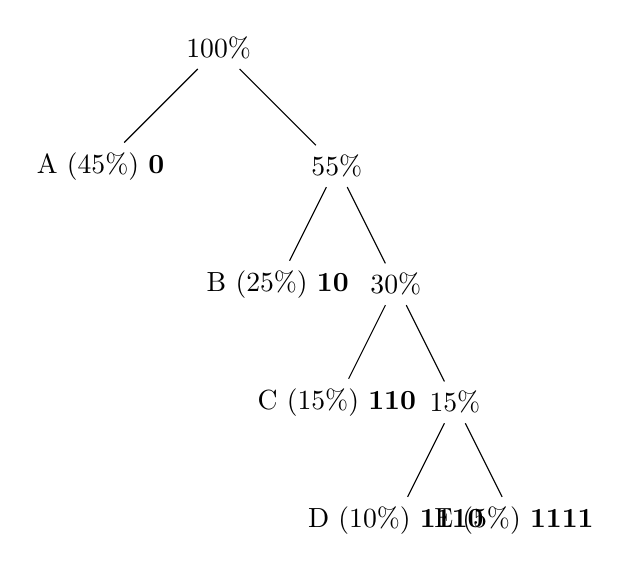
\begin{tikzpicture}[level distance=1.5cm, level 1/.style={sibling distance=3cm}, level 2/.style={sibling distance=1.5cm}]
    \node {100\%}
        child {node {A (45\%) \textbf{0}}}
        child {node {55\%}
            child {node {B (25\%) \textbf{10}}}
            child {node {30\%}
                child {node {C (15\%) \textbf{110}}}
                child {node {15\%}
                    child {node {D (10\%) \textbf{1110}}}
                    child {node {E (5\%) \textbf{1111}}}
                }
            }
        };
\end{tikzpicture}
\captionof{figure}{Huffman Tree}
\end{center}

\textbf{Shannon-Fano Code:}
Shannon-Fano algorithm recursively divides symbols into two groups of similar frequency, then assigns 0 to one group and 1 to the other.

\textbf{Shannon-Fano Tree:}
\begin{center}
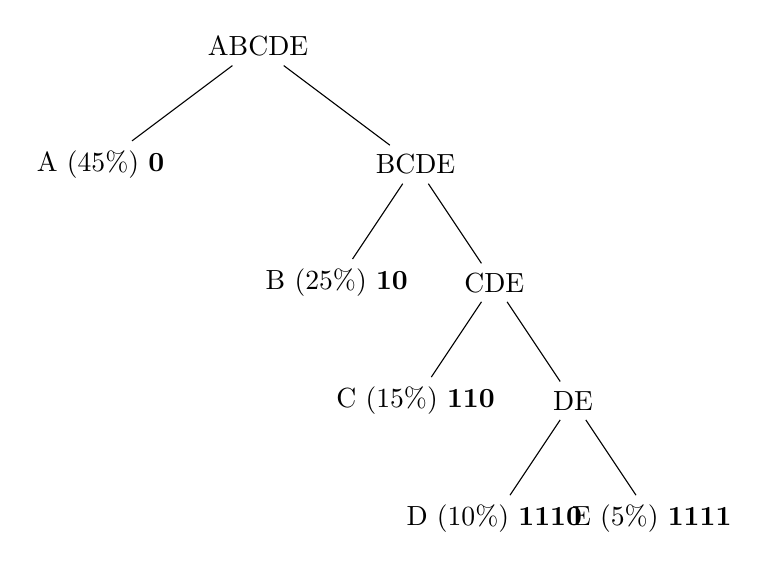
\begin{tikzpicture}[level distance=1.5cm, level 1/.style={sibling distance=4cm}, level 2/.style={sibling distance=2cm}]
    \node {ABCDE}
        child {node {A (45\%) \textbf{0}}}
        child {node {BCDE}
            child {node {B (25\%) \textbf{10}}}
            child {node {CDE}
                child {node {C (15\%) \textbf{110}}}
                child {node {DE}
                    child {node {D (10\%) \textbf{1110}}}
                    child {node {E (5\%) \textbf{1111}}}
                }
            }
        };
\end{tikzpicture}
\captionof{figure}{Shannon-Fano Tree}
\end{center}
\end{solutionbox}

\begin{mnemonicbox}
\mnemonic{FREDS - Frequency Reduces Encoding Digit Size}
\end{mnemonicbox}

\questionmarks{3(a OR)}{3}{State the features of RS-232.}

\begin{solutionbox}
\begin{center}
\captionof{table}{Features of RS-232}
\begin{tabulary}{\linewidth}{|L|}
\hline
\textbf{Features of RS-232} \\ \hline
\textbf{Single-ended signaling} \\ \hline
\textbf{Maximum data rate} of 20 kbps \\ \hline
\textbf{Maximum cable length} of 15 meters \\ \hline
\textbf{Point-to-point communication} (1 driver, 1 receiver) \\ \hline
\textbf{Voltage levels}: -15V to +15V \\ \hline
\textbf{25-pin or 9-pin} DB connector standard \\ \hline
\end{tabulary}
\end{center}
\end{solutionbox}

\begin{mnemonicbox}
\mnemonic{SMPVD - Single Maximum Point-to-point Voltage DB-connector}
\end{mnemonicbox}

\questionmarks{3(b OR)}{4}{What is channel capacity in terms of SNR? Explain its importance.}

\begin{solutionbox}
\textbf{Channel Capacity:}
The maximum rate at which information can be transmitted over a communication channel with an arbitrarily small probability of error.

\textbf{Formula:} $C = B \times \log_2(1 + SNR)$
Where: C = Channel capacity (bps), B = Bandwidth (Hz), SNR = Signal-to-Noise Ratio.

\begin{center}
\captionof{table}{Importance}
\begin{tabulary}{\linewidth}{|L|}
\hline
\textbf{Importance of Channel Capacity} \\ \hline
\textbf{Sets theoretical limits} for data transmission \\ \hline
\textbf{Guides system design} and optimization \\ \hline
\textbf{Helps evaluate performance} of communication systems \\ \hline
\textbf{Determines required bandwidth} for a given data rate \\ \hline
\textbf{Informs coding techniques} to approach capacity \\ \hline
\end{tabulary}
\end{center}

\begin{center}
\begin{tikzpicture}[node distance=2cm, auto]
    \node [gtu block] (bw) {Bandwidth};
    \node [gtu block, below=1cm of bw] (snr) {SNR};
    \node [gtu block, right=2cm of bw, yshift=-0.5cm] (cap) {Channel Capacity};
    \node [gtu block, right=1.5cm of cap] (rate) {Max Data Rate};
    
    \draw [gtu arrow] (bw) -- (cap);
    \draw [gtu arrow] (snr) -- (cap);
    \draw [gtu arrow] (cap) -- (rate);
\end{tikzpicture}
\captionof{figure}{Channel Capacity Factors}
\end{center}
\end{solutionbox}

\begin{mnemonicbox}
\mnemonic{BSNR - Bandwidth and SNR Need Relationship}
\end{mnemonicbox}

\questionmarks{3(c OR)}{7}{Explain in detail any one error detection and error correction technique in digital communication.}

\begin{solutionbox}
\textbf{Hamming Code Error Detection and Correction:}
Hamming code is a linear error-correcting code that can detect and correct single-bit errors. 
\begin{itemize}
    \item Data bits are at powers of 2 positions not used by parity.
    \item Parity bits are at positions 1, 2, 4, 8...
\end{itemize}

\textbf{Example: 7-bit Hamming code (4 data, 3 parity)}
\begin{center}
\captionof{table}{Hamming Code Structure}
\begin{tabulary}{\linewidth}{|C|C|C|C|C|C|C|C|}
\hline
\textbf{Position} & 1 & 2 & 3 & 4 & 5 & 6 & 7 \\ \hline
\textbf{Bit Type} & P1 & P2 & D1 & P4 & D2 & D3 & D4 \\ \hline
\end{tabulary}
\end{center}

\textbf{Parity Bit Calculation:}
\begin{itemize}
    \item P1 checks 1, 3, 5, 7.
    \item P2 checks 2, 3, 6, 7.
    \item P4 checks 4, 5, 6, 7.
\end{itemize}

\textbf{Error Correction:}
Parity checks indicate error position (binary value of P4 P2 P1 gives position).

\begin{center}
\captionof{table}{Error Location}
\begin{tabulary}{\linewidth}{|C|C|C|L|}
\hline
\textbf{P4} & \textbf{P2} & \textbf{P1} & \textbf{Error Position} \\ \hline
0 & 0 & 0 & No error \\ \hline
0 & 0 & 1 & Position 1 \\ \hline
1 & 0 & 1 & Position 5 \\ \hline
1 & 1 & 1 & Position 7 \\ \hline
\end{tabulary}
\end{center}
\end{solutionbox}

\begin{mnemonicbox}
\mnemonic{PECD - Parity Enables Correction of Data}
\end{mnemonicbox}

\questionmarks{4(a)}{3}{Draw the block diagram of satellite communication and explain in brief.}

\begin{solutionbox}
\begin{center}
\begin{tikzpicture}[node distance=2.5cm, auto]
    \node [gtu block] (gs1) {Ground Station 1};
    \node [gtu block, right=4cm of gs1] (gs2) {Ground Station 2};
    \node [gtu block, above=2cm of $(gs1)!0.5!(gs2)$] (sat) {Satellite};
    
    \draw [gtu arrow, bend left] (gs1) to node {Uplink} (sat);
    \draw [gtu arrow, bend left] (sat) to node {Downlink} (gs2);
    
    \node [left=0.5cm of gs1] (tx) {Transmitter};
    \node [right=0.5cm of gs2] (rx) {Receiver};
    
    \draw [gtu arrow] (tx) -- (gs1);
    \draw [gtu arrow] (gs2) -- (rx);
\end{tikzpicture}
\captionof{figure}{Satellite Communication}
\end{center}

\textbf{Explanation:}
Satellite communication involves transmitting signals from an Earth station to a satellite (uplink), which amplifies and retransmits them to Earth (downlink).

\textbf{Key Components:}
\begin{itemize}
    \item \keyword{Earth Stations}: Transmit/Receive signals.
    \item \keyword{Transponders}: Satellite repeaters.
\end{itemize}
\end{solutionbox}

\begin{mnemonicbox}
\mnemonic{STAR - Satellite Transmits And Receives}
\end{mnemonicbox}

\questionmarks{4(b)}{4}{Sketch the Unipolar NRZ, Polar RZ, Polar NRZ and AMI waveform for 10101101 data sequence.}

\begin{solutionbox}
\begin{center}
\begin{tikzpicture}[x=0.8cm,y=0.6cm]
    % Data: 1 0 1 0 1 1 0 1
    \node[anchor=east] at (-1, 1) {Data:};
    \foreach \x/\val in {0/1, 1/0, 2/1, 3/0, 4/1, 5/1, 6/0, 7/1} {
        \draw (\x,0) -- (\x,\val) -- (\x+1,\val) -- (\x+1,0); 
        \node at (\x+0.5, 1.5) {\val};
    }
    
    % Unipolar NRZ (1: High, 0: 0)
    \node[anchor=east] at (-1, -1.5) {Unipolar NRZ:};
    \draw (0,-1.5) -- (0, -0.5) -- (1,-0.5) -- (1,-1.5) -- (2,-1.5) -- (2,-0.5) -- (3,-0.5) -- (3,-1.5) -- (4,-1.5) -- (4,-0.5) -- (6,-0.5) -- (6,-1.5) -- (7,-1.5) -- (7,-0.5) -- (8,-0.5);
    
    % Polar RZ (1: +V half, 0: -V half? Or just 1 return to zero? Typical Polar RZ: 1 -> +V/0, 0 -> -V/0)
    % Assuming standard Polar RZ: 1 is +V for half, 0 is -V for half.
    \node[anchor=east] at (-1, -4) {Polar RZ:};
    \foreach \x/\val in {0/1, 1/-1, 2/1, 3/-1, 4/1, 5/1, 6/-1, 7/1} {
        \draw (\x,-4) -- (\x, -4+\val) -- (\x+0.5,-4+\val) -- (\x+0.5,-4) -- (\x+1,-4);
    }
    
    % Polar NRZ (1: +V, 0: -V)
    \node[anchor=east] at (-1, -6.5) {Polar NRZ:};
    \draw (0,-6.5) -- (0, -5.5) -- (1,-5.5) -- (1,-7.5) -- (2,-7.5) -- (2,-5.5) -- (3,-5.5) -- (3,-7.5) -- (4,-7.5) -- (4,-5.5) -- (6,-5.5) -- (6,-7.5) -- (7,-7.5) -- (7,-5.5) -- (8,-5.5);

    % AMI (Alt Mark Inversion: 1 alt pol, 0 zero)
    \node[anchor=east] at (-1, -9) {AMI:};
    % 1(+), 0, 1(-), 0, 1(+), 1(-), 0, 1(+)
    \draw (0,-9) -- (0, -8) -- (1,-8) -- (1,-9) -- (2,-9) -- (2,-10) -- (3,-10) -- (3,-9) -- (4,-9) -- (4,-8) -- (5,-8) -- (5,-9) -- (5,-10) -- (6,-10) -- (6,-9) -- (7,-9) -- (7,-8) -- (8,-8);
    
\end{tikzpicture}
\captionof{figure}{Line Coding Waveforms}
\end{center}
\end{solutionbox}

\begin{mnemonicbox}
\mnemonic{UPPA - Unipolar Polar Polar AMI}
\end{mnemonicbox}

\questionmarks{4(c)}{7}{Explain data transmission techniques in details with suitable example for digital communication.}

\begin{solutionbox}
\textbf{Data Transmission Techniques:}
\begin{center}
\captionof{table}{Techniques}
\begin{tabulary}{\linewidth}{|L|L|L|}
\hline
\textbf{Technique} & \textbf{Description} & \textbf{Example} \\ \hline
\textbf{Serial} & Data bits sent one after another over single channel & USB, UART \\ \hline
\textbf{Parallel} & Multiple bits sent simultaneously over multiple channels & Printer, SCSI \\ \hline
\textbf{Synchronous} & Continuous stream with timing signals & Ethernet \\ \hline
\textbf{Asynchronous} & Start/stop bits used & RS-232 \\ \hline
\end{tabulary}
\end{center}

\textbf{Serial Transmission (UART Example):}
\begin{center}
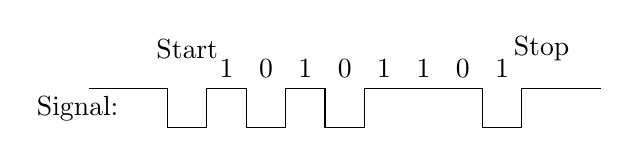
\begin{tikzpicture}[x=0.5cm, y=0.5cm]
    \node[anchor=east] at (-1, 0.5) {Signal:};
    % Start(0), 1, 0, 1, 0, 1, 1, 0, 1, Stop(1)
    % Idle is usually 1. Start drops to 0.
    \draw (-2,1) -- (0,1) -- (0,0) -- (1,0) -- (1,1) -- (2,1) -- (2,0) -- (3,0) -- (3,1) -- (4,1) -- (4,0) -- (5,0) -- (5,1) -- (6,1) -- (7,1) -- (8,1) -- (8,0) -- (9,0) -- (9,1) -- (10,1) -- (11,1);
    \node at (0.5, 2) {Start};
    \node at (9.5, 2) {Stop};
    \foreach \x/\v in {1/1, 2/0, 3/1, 4/0, 5/1, 6/1, 7/0, 8/1} {
        \node at (\x+0.5, 1.5) {\v};
    }
\end{tikzpicture}
\captionof{figure}{Serial Transmission}
\end{center}

\textbf{Parallel Transmission:}
\begin{center}
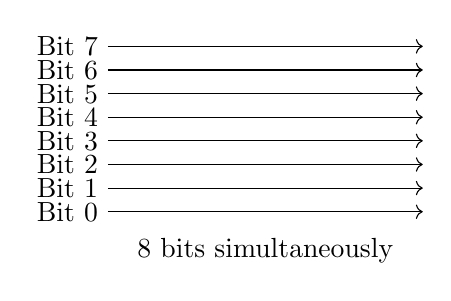
\begin{tikzpicture}
    \foreach \y in {0,1,2,3,4,5,6,7} {
        \draw[->] (0,\y*0.3) -- (4,\y*0.3);
        \node[left] at (0,\y*0.3) {Bit \y};
    }
    \node at (2, -0.5) {8 bits simultaneously};
\end{tikzpicture}
\captionof{figure}{Parallel Transmission}
\end{center}
\end{solutionbox}

\begin{mnemonicbox}
\mnemonic{SPASH - Serial Parallel Asynchronous Synchronous Half-duplex}
\end{mnemonicbox}

\questionmarks{4(a OR)}{3}{Interpret the aspects of spread spectrum techniques.}

\begin{solutionbox}
\begin{center}
\captionof{table}{Spread Spectrum Aspects}
\begin{tabulary}{\linewidth}{|L|L|}
\hline
\textbf{Aspect} & \textbf{Interpretation} \\ \hline
\textbf{Bandwidth Spreading} & Signal spread over wider bandwidth \\ \hline
\textbf{Security} & Difficult to intercept/jam \\ \hline
\textbf{Noise Immunity} & Resistant to narrowband interference \\ \hline
\textbf{Multiple Access} & Allows sharing of frequency \\ \hline
\textbf{Low Power Density} & Signal appears as noise \\ \hline
\end{tabulary}
\end{center}

\begin{center}
\begin{tikzpicture}[node distance=2cm, auto]
    \node [gtu block] (nb) {Narrow Band};
    \node [gtu block, right=2cm of nb] (spread) {Spreading};
    \node [gtu block, right=2cm of spread] (wb) {Wideband};
    \node [gtu block, below=1cm of spread] (code) {Code};
    
    \draw [gtu arrow] (nb) -- (spread);
    \draw [gtu arrow] (spread) -- (wb);
    \draw [gtu arrow] (code) -- (spread);
\end{tikzpicture}
\captionof{figure}{Spread Spectrum Concept}
\end{center}
\end{solutionbox}

\begin{mnemonicbox}
\mnemonic{BSNML - Bandwidth Security Noise Multiple Low-power}
\end{mnemonicbox}

\questionmarks{4(b OR)}{4}{Write a short note on probability and discuss its properties for digital communication.}

\begin{solutionbox}
\textbf{Probability:} Foundation for analyzing error rates and reliability.

\begin{center}
\captionof{table}{Properties}
\begin{tabulary}{\linewidth}{|L|L|L|}
\hline
\textbf{Property} & \textbf{Description} & \textbf{Relevance} \\ \hline
\textbf{Range} & $0 \le P(E) \le 1$ & Bounds for error prob \\ \hline
\textbf{Certainty} & $P(S) = 1$ & Total prob \\ \hline
\textbf{Additivity} & $P(A \cup B) = P(A) + P(B)$ & Total error rate \\ \hline
\textbf{Conditional} & $P(A|B)$ & Channel modeling \\ \hline
\textbf{Independence} & $P(A \cap B) = P(A)P(B)$ & Uncorrelated noise \\ \hline
\end{tabulary}
\end{center}
\end{solutionbox}

\begin{mnemonicbox}
\mnemonic{RACIC - Range Additivity Certainty Independence Conditional}
\end{mnemonicbox}

\questionmarks{4(c OR)}{7}{Explain Data transmission mode in details with example.}

\begin{solutionbox}
\textbf{Data Transmission Modes:}

\begin{center}
\captionof{table}{Modes}
\begin{tabulary}{\linewidth}{|L|L|L|}
\hline
\textbf{Mode} & \textbf{Description} & \textbf{Example} \\ \hline
\textbf{Simplex} & One-way only & TV, Radio \\ \hline
\textbf{Half-Duplex} & Two-way, one at a time & Walkie-talkie \\ \hline
\textbf{Full-Duplex} & Two-way simultaneous & Telephone \\ \hline
\end{tabulary}
\end{center}

\begin{center}
\begin{tikzpicture}[node distance=2cm, auto]
    % Simplex
    \node [gtu block] (tx1) {Tx};
    \node [gtu block, right=1.5cm of tx1] (rx1) {Rx};
    \draw [gtu arrow] (tx1) -- node {Simplex} (rx1);
    
    % Half Duplex
    \node [gtu block, below=1.5cm of tx1] (devA) {Dev A};
    \node [gtu block, right=1.5cm of devA] (devB) {Dev B};
    \draw [gtu arrow, bend left] (devA) to node {Time 1} (devB);
    \draw [gtu arrow, bend left] (devB) to node {Time 2} (devA);
    \node at ($(devA)!0.5!(devB) + (0,-1)$) {Half-Duplex};
    
    % Full Duplex
    \node [gtu block, below=3cm of tx1] (devA2) {Dev A};
    \node [gtu block, right=1.5cm of devA2] (devB2) {Dev B};
    \draw [gtu arrow, transform canvas={yshift=0.1cm}] (devA2) -- node {Ch 1} (devB2);
    \draw [gtu arrow, transform canvas={yshift=-0.1cm}] (devB2) -- node {Ch 2} (devA2);
    \node at ($(devA2)!0.5!(devB2) + (0,-0.8)$) {Full-Duplex};
\end{tikzpicture}
\captionof{figure}{Transmission Modes}
\end{center}
\end{solutionbox}

\begin{mnemonicbox}
\mnemonic{SHF - Simplex Half Full}
\end{mnemonicbox}

\questionmarks{5(a)}{3}{Explain Edge Computing in detail.}

\begin{solutionbox}
\textbf{Edge Computing:} Distributed computing bringing computation closer to data sources.

\begin{center}
\captionof{table}{Key Aspects}
\begin{tabulary}{\linewidth}{|L|L|}
\hline
\textbf{Aspect} & \textbf{Description} \\ \hline
\textbf{Decentralization} & Processing at network edge \\ \hline
\textbf{Reduced Latency} & Faster response \\ \hline
\textbf{Bandwidth Efficiency} & Less data to cloud \\ \hline
\textbf{Security} & Sensitive data remains local \\ \hline
\end{tabulary}
\end{center}

\begin{center}
\begin{tikzpicture}[node distance=2cm, auto]
    \node [gtu block] (iot) {IoT Devices};
    \node [gtu block, right=2cm of iot] (edge) {Edge Computing};
    \node [gtu block, right=2cm of edge, yshift=1cm] (local) {Local Processing};
    \node [gtu block, right=2cm of edge, yshift=-1cm] (cloud) {Cloud};
    
    \draw [gtu arrow] (iot) -- (edge);
    \draw [gtu arrow] (edge) -- (local);
    \draw [gtu arrow] (edge) -- (cloud);
\end{tikzpicture}
\captionof{figure}{Edge Computing Architecture}
\end{center}
\end{solutionbox}

\begin{mnemonicbox}
\mnemonic{DRBLES - Decentralized Reduces Bandwidth, Latency, Exposure, Strengthens reliability}
\end{mnemonicbox}

\questionmarks{5(b)}{4}{Enlist the features of 5G Technology in data communication.}

\begin{solutionbox}
\begin{center}
\captionof{table}{Features of 5G}
\begin{tabulary}{\linewidth}{|L|}
\hline
\textbf{Features of 5G Technology} \\ \hline
\textbf{High Data Rates} (up to 20 Gbps peak) \\ \hline
\textbf{Ultra-Low Latency} (1 ms or less) \\ \hline
\textbf{Massive Device Connectivity} (1M devices per km$^2$) \\ \hline
\textbf{Network Slicing} (customized virtual networks) \\ \hline
\textbf{Beamforming} (directed signal transmission) \\ \hline
\textbf{Millimeter Wave Spectrum} (24-100 GHz) \\ \hline
\end{tabulary}
\end{center}

\begin{center}
\begin{tikzpicture}[node distance=2cm, auto]
    \node [gtu block] (5g) {5G Technology};
    \node [gtu block, right=2cm of 5g, yshift=1.5cm] (embb) {eMBB};
    \node [gtu block, right=2cm of 5g] (urllc) {URLLC};
    \node [gtu block, right=2cm of 5g, yshift=-1.5cm] (mmtc) {mMTC};
    
    \draw [gtu arrow] (5g) -- (embb);
    \draw [gtu arrow] (5g) -- (urllc);
    \draw [gtu arrow] (5g) -- (mmtc);
\end{tikzpicture}
\captionof{figure}{5G Use Cases}
\end{center}
\end{solutionbox}

\begin{mnemonicbox}
\mnemonic{HUMBLE-MN - High-speed Ultra-low-latency Massive Beamforming Low-latency Enhanced Millimeter Network}
\end{mnemonicbox}

\questionmarks{5(c)}{7}{Write a details note on Data communication including its characteristics and components.}

\begin{solutionbox}
\textbf{Data Communication:} Process of transferring digital information.

\textbf{Characteristics:}
\begin{itemize}
    \item \keyword{Delivery}: Correct destination.
    \item \keyword{Accuracy}: No errors.
    \item \keyword{Timeliness}: On time.
    \item \keyword{Jitter}: Consistent timing.
    \item \keyword{Security}: Protected access.
\end{itemize}

\textbf{Components:}
\begin{center}
\captionof{table}{Components}
\begin{tabulary}{\linewidth}{|L|L|}
\hline
\textbf{Component} & \textbf{Description} \\ \hline
\textbf{Message} & Information to be communicated \\ \hline
\textbf{Sender} & Device sending data \\ \hline
\textbf{Receiver} & Device receiving data \\ \hline
\textbf{Medium} & Physical path \\ \hline
\textbf{Protocol} & Rules governing communication \\ \hline
\end{tabulary}
\end{center}

\begin{center}
\begin{tikzpicture}[node distance=1.5cm, auto]
    \node [gtu block] (sender) {Sender};
    \node [gtu block, right=1cm of sender] (enc) {Encoder};
    \node [gtu block, right=1cm of enc] (med) {Medium};
    \node [gtu block, right=1cm of med] (dec) {Decoder};
    \node [gtu block, right=1cm of dec] (rx) {Receiver};
    
    \node [gtu block, above=1cm of med] (proto) {Protocol};
    
    \draw [gtu arrow] (sender) -- (enc);
    \draw [gtu arrow] (enc) -- (med);
    \draw [gtu arrow] (med) -- (dec);
    \draw [gtu arrow] (dec) -- (rx);
    
    \draw [dashed] (proto) -- (sender);
    \draw [dashed] (proto) -- (enc);
    \draw [dashed] (proto) -- (med);
    \draw [dashed] (proto) -- (dec);
    \draw [dashed] (proto) -- (rx);
\end{tikzpicture}
\captionof{figure}{Data Communication Model}
\end{center}
\end{solutionbox}

\begin{mnemonicbox}
\mnemonic{DATJS-MSRTP - Delivery Accuracy Timeliness Jitter Security - Message Sender Receiver Transmission Protocol}
\end{mnemonicbox}

\questionmarks{5(a OR)}{3}{Identify and write privacy consideration in Data communication.}

\begin{solutionbox}
\begin{itemize}
    \item \keyword{Data Encryption}: Protecting data during transmission.
    \item \keyword{Access Control}: Only authorized users.
    \item \keyword{Authentication}: Verifying identity.
    \item \keyword{Data Minimization}: Collecting only necessary data.
    \item \keyword{End-to-End Security}: Protection throughout path.
\end{itemize}

\begin{center}
\begin{tikzpicture}[node distance=2cm, auto]
    \node [gtu block] (priv) {Privacy};
    \node [gtu block, right=2cm of priv, yshift=1cm] (enc) {Encryption};
    \node [gtu block, right=2cm of priv] (auth) {Authentication};
    \node [gtu block, right=2cm of priv, yshift=-1cm] (access) {Access Control};
    
    \draw [gtu arrow] (priv) -- (enc);
    \draw [gtu arrow] (priv) -- (auth);
    \draw [gtu arrow] (priv) -- (access);
\end{tikzpicture}
\captionof{figure}{Privacy Considerations}
\end{center}
\end{solutionbox}

\begin{mnemonicbox}
\mnemonic{DAAESE - Data is Authenticated, Accessed, Encrypted Securely End-to-end}
\end{mnemonicbox}

\questionmarks{5(b OR)}{4}{What is block chain in communication security? Enlist its features.}

\begin{solutionbox}
\textbf{Blockchain:} Distributed ledger technology providing secure, tamper-proof records.

\begin{center}
\captionof{table}{Features}
\begin{tabulary}{\linewidth}{|L|L|}
\hline
\textbf{Feature} & \textbf{Description} \\ \hline
\textbf{Decentralization} & No central authority \\ \hline
\textbf{Immutability} & Cannot be altered \\ \hline
\textbf{Transparency} & Visible to participants \\ \hline
\textbf{Cryptographic Security} & Secured using crypto \\ \hline
\textbf{Consensus} & Network agreement \\ \hline
\end{tabulary}
\end{center}

\begin{center}
\begin{tikzpicture}[node distance=1.5cm, auto]
    \node [gtu block] (b1) {Block 1};
    \node [gtu block, right=1cm of b1] (b2) {Block 2};
    \node [gtu block, right=1cm of b2] (b3) {Block 3};
    
    \draw [gtu arrow] (b1) -- node {Hash} (b2);
    \draw [gtu arrow] (b2) -- node {Hash} (b3);
\end{tikzpicture}
\captionof{figure}{Blockchain Structure}
\end{center}
\end{solutionbox}

\begin{mnemonicbox}
\mnemonic{DITCSD - Decentralized Immutable Transparent Cryptographic Secure Distributed}
\end{mnemonicbox}

\questionmarks{5(c OR)}{7}{Write and illustrate different communication ports: USB, HDMI, RCA and Ethernet.}

\begin{solutionbox}
\textbf{Communication Ports:}

\begin{enumerate}
    \item \textbf{USB (Universal Serial Bus)}: Data/Power, 40 Gbps, Hot-swappable.
    \item \textbf{HDMI}: Audio/Video, 48 Gbps, HDCP.
    \item \textbf{RCA}: Analog Audio/Video, Colored (Red/White/Yellow).
    \item \textbf{Ethernet (RJ-45)}: Network, 10 Gbps, Twisted pair.
\end{enumerate}

\begin{center}
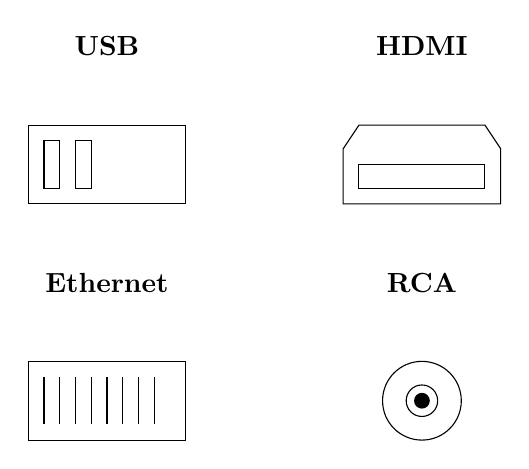
\begin{tikzpicture}
    % USB
    \node at (0, 2) {\textbf{USB}};
    \draw (-1,0) rectangle (1,1);
    \draw (-0.8, 0.2) rectangle (-0.6, 0.8);
    \draw (-0.4, 0.2) rectangle (-0.2, 0.8);
    
    % HDMI
    \node at (4, 2) {\textbf{HDMI}};
    \draw (3,0) -- (5,0) -- (5,0.7) -- (4.8, 1) -- (3.2, 1) -- (3, 0.7) -- cycle;
    \draw (3.2, 0.2) rectangle (4.8, 0.5);
    
    % RJ45
    \node at (0, -1) {\textbf{Ethernet}};
    \draw (-1,-3) rectangle (1,-2);
    \foreach \x in {-0.8, -0.6, -0.4, -0.2, 0, 0.2, 0.4, 0.6}
        \draw (\x, -2.8) -- (\x, -2.2);
        
    % RCA
    \node at (4, -1) {\textbf{RCA}};
    \draw (4,-2.5) circle (0.5);
    \draw (4,-2.5) circle (0.2);
    \fill (4,-2.5) circle (0.1);
\end{tikzpicture}
\captionof{figure}{Port Illustrations}
\end{center}

\begin{center}
\captionof{table}{Comparison}
\begin{tabulary}{\linewidth}{|L|L|L|L|}
\hline
\textbf{Port} & \textbf{Type} & \textbf{Max Speed} & \textbf{Use} \\ \hline
\textbf{USB} & Digital & 40 Gbps & Data/Power \\ \hline
\textbf{HDMI} & Digital & 48 Gbps & Audio/Video \\ \hline
\textbf{RCA} & Analog & Low & Audio/Video \\ \hline
\textbf{Ethernet} & Digital & 10 Gbps & Network \\ \hline
\end{tabulary}
\end{center}
\end{solutionbox}

\begin{mnemonicbox}
\mnemonic{UHRE - USB Handles Rapid Ethernet, HDMI Delivers Rich Entertainment}
\end{mnemonicbox}

\end{document}

